\chapter{Termodinámica}

\textit{La termodinámica es el estudio de las restricciones a las posibles propiedades de la materia que se derivan de las propiedades de simetría de las leyes fundamentales de la física.}

\section{Conceptos Básicos}

\paragraph{Propósito: } La termodinámica busca describir sistemas de muchas partículas ($10^{23}$ típicamente). Gases, líquidos, cristales, estrellas, universo, \ldots ,  \underline{sistemas macroscópicos} y en particular, estudiar los procesos de transferencia de energía (trabajo y calor) entre cuerpos macroscópicos\footnote{Más adelante se tratará la parte microscópica con la Mecánica Estadística, poder explicativo y predictivo sobre propiedades macroscópicas de la materia, partiendo de una descripción microscópica.}. 

\begin{itemize}
	\item Definir cantidades físicas, "variables de estado" que caracterizan un sistema macroscópico: $V,T,N,U,\ldots$.
	\item Relacionar estas cantidades entre sí:
		\begin{enumerate}
			\item Válidas para cualquier sistema en equilibrio:
			\begin{enumerate}
				\item Leyes axiomáticas de la termodinámica, como Ley de la Energía, Ley de la Entroía, etc.
			\end{enumerate}
			\item Específicas
			\begin{enumerate}
				\item Por ecuaciones de estado como: fenomenológicas, empíricas, experimentales en la mayoria de los casos.
			\end{enumerate}
		\end{enumerate}
\end{itemize}


Es importante mencionar que la termodinámica clásica macroscópica no puede explicar porqué una ecuación de estado describe un sistema partícular.



\section{Sistemas Termodinámicos y Cantidades de Estado}

\begin{enumerate}
	\item Sistema Termodinámico:
	\begin{figure}[H]
		\centering
		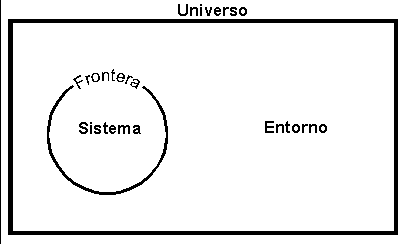
\includegraphics[scale=0.3]{./img/thermodynamicSystem.png}
		\label{thermodynamicSystem}
		\caption{Representación gráfica de las partes de un sistema termodinámico.}
	\end{figure}
	
	\item Tipos de Sistemas: (depende de la frontera)
	\begin{itemize}
		\item Sistemas aislados: No intercambian energía con el entorno.
		\item Sistemas cerrados
	\end{itemize}
\end{enumerate}






